\documentclass[crop,tikz]{standalone}

\usepackage{tikz}
\usepackage{circuitikz}
\usetikzlibrary{circuits.logic.US}

\begin{document}
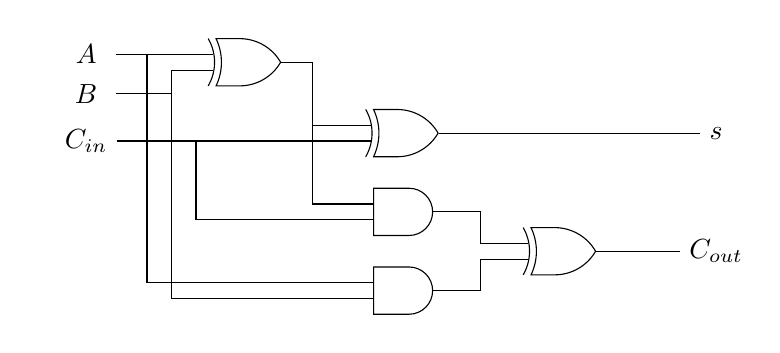
\begin{tikzpicture}[%
          circuit logic US,
          tiny circuit symbols,
          every circuit symbol/.style={fill=white, draw},
          node distance=3mm and 0mm,
          branch/.style={fill,shape=circle,minimum size=3pt,inner sep=0pt}]

  \node (a) at (0, 2) { $~A~$ };
  \node (b) at (0, 1.5) { $~B~$ };
  \node (cin) at (0, 0.9) { $C_{in}$ };

  \node (invisible1) at (0, 2.1) { \phantom{invisible} };
  \node (invisible2) at (0, -1.2) { \phantom{invisible} };

  \node (s) at (8, 1) { $s$ };
  \node (cout) at (8, -0.5) { $C_{out}$ };

  \node[xor gate,minimum size=0.6cm] at ($(2,1.90)$) (xor1) {};
  \node[xor gate,minimum size=0.6cm] at ($(4,1)$) (xor2) {};
  \node[and gate,minimum size=0.6cm] at ($(4,0)$) (and1) {};
  \node[and gate,minimum size=0.6cm] at ($(4,-1)$) (and2) {};
  \node[xor gate,minimum size=0.6cm] at ($(6,-0.5)$) (xor3) {};

  \draw (a.east) --++(180:-4mm) |- (xor1.input 1);
  \draw (b.east) --++(180:-7mm) |- (xor1.input 2);
  \draw (xor1.output) --++(180:-4mm) |- (xor2.input 1);
  \draw (cin.east) |- (xor2.input 2);

  \draw (a.east) --++(180:-4mm) |- (and2.input 1);
  \draw (b.east) --++(180:-7mm) |- (and2.input 2);

  \draw (xor1.output) --++(180:-4mm) |- (and1.input 1);
  \draw (cin.east) --++(180:-10mm)    |- (and1.input 2);

  \draw (and1.output) --++(180:-6mm) |- (xor3.input 1);
  \draw (and2.output) --++(180:-6mm) |- (xor3.input 2);

  \draw (xor2.output) |- (s.west);
  \draw (xor3.output) |- (cout.west);

\end{tikzpicture}
\end{document}
